% Target: 4-6 blz
\epigraph{You're the chosen one, Cuckoo.}{Adriaan}

For the Proof of Concept (PoC), Cuckoo \cite{cuckoo} was choosen. \todo{Explanation of Cuckoo...}\\

Cuckoo was choosen because it more or less already implemented steps one and two of our algorithm. Cuckoo, through Cuckoomon \cite{cuckoomon}, provides a series of hooks which monitor calls between the browser and the operating system. This allows us to monitor the extra information from section \ref{algo2}. These hooks, conveniently, also monitor the network calls made by the browser and thus we are able to read the network traffic from the browser.\\

Besides of the encountered problems, explained in section \ref{99problems}, Cuckoo has the disavantage that it only supports Microsoft Windows as a sandbox. However, as this was only a PoC with limited time to implement, it was decided that the avantages outweigh the disavantages and thus Cuckoo was choosen as the base for our generic algorithm. Additionaly, only Internet Explorer has been implemented as a supported browser.

\subsubsection{Step 1}

Internet Explorer uses the operating system to encrypt HTTP requests and decrypt HTTP responses. The security support provider (SSP) who is responsible for this is called ``Schannel'' or ``Secure Channel''\cite{schannel}. This allowed us to monitor traffic on the operating system level without any need for a proxy to decrypt the traffic.

\subsubsection{Step 2}

As already explained, Cuckoo uses Cuckoomon, which uses hooks to monitor calls, to keep track of the browser activity. Besides adding a few new hooks and deleting a few irrelevant hooks for drive-by downloads, nothing major was changed to Cuckoomon.

\subsubsection{Step 3}

To allow for concurrently visiting multiple websites in one sandbox environment, Cuckoo had to be extended to allow this as the current development version only accepts one URL at a time. Although, support for this was added pretty quickly using tabs, this left us with a problem to detect when a new URL was feeded to a tab\todo{See problems below}. To solve this problem, every URL is now opened in its own window.

\subsubsection{Step 4}

10 events were defined 

\begin{description}
\item[on\_process\_new] sfdsfdf
\item[on\_process\_finished] sfdsfdf
\item[on\_http\_request] sfdsfdf
\item[on\_file\_write] sfdsfdf
\item[on\_file\_delete] sfdsfdf
\item[on\_registry\_set] sfdsfdf
\item[on\_registry\_delete] sfdsfdf
\item[on\_shell\_execute] sfdsfdf
\item[on\_socket\_connect] sfdsfdf
\item[on\_anomaly\_detected] sfdsfdf
\end{description}

\subsubsection{Step 5}

The events are put in the graph
See figure \ref{fig:alg_tree}. \todo{Explain the colors of the vertices}

Figure \ref{fig:alg_tree} also shows a website with a drive-by download. In the top left, one can see process spawns (red vertices) in an unusual place.\todo{beter uitleggen}

\begin{figure}[h]
    \centering
    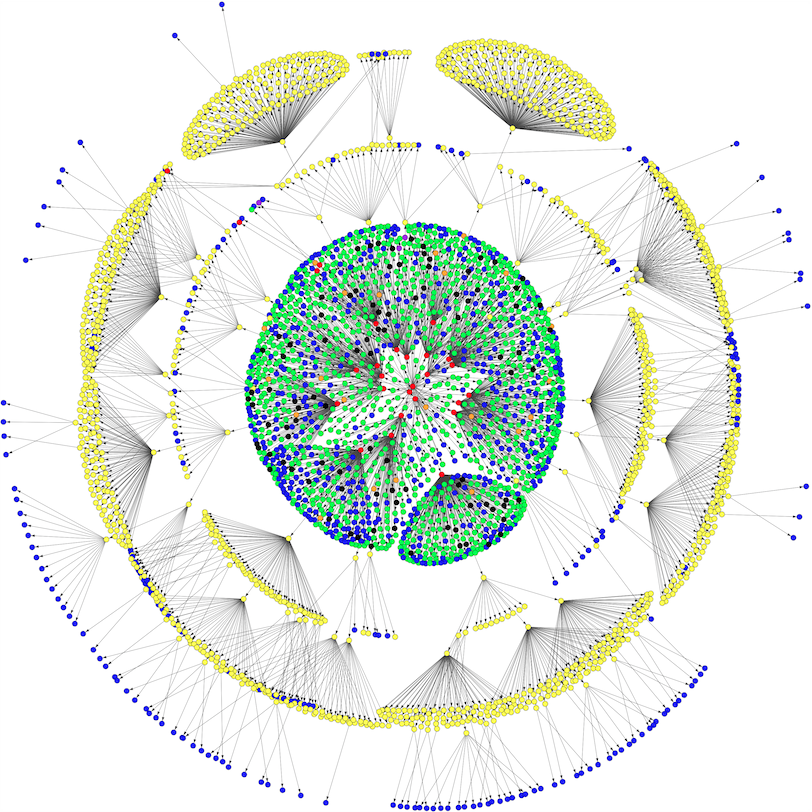
\includegraphics[width=17cm]{Images/graph2.png}
    \caption{An example of the graph}
    \label{fig:alg_tree}
\end{figure}
\subsubsection{Step 6}

For this Proof of Concept, one Analyzer was written which searches the graph for unusual places where processes are spawned. All processes which are spawned and are a child process of a Internet Explorer window are flagged and in Step 7 reported to the user.


\subsubsection{Step 7}

\todo{Betere analyzer reporting in output script...}
\begin{lstlisting}
$ utils/mass-analyse.py -g -t 22
Warning: Task with ID 22 is not yet completed; Waiting...
INFO:root:Parse log....
Analyzer 'Subprocess_from_tab': The URL 'http://camhogger.com' spawns a process called 'errfix.exe'.
\end{lstlisting}

\subsubsection{Improvements}

\todo{Speedboost tussen Cuckoo 1.2-dev en onze wijzigingen in grafiekje zetten}



\subsubsection{Problems}
\label{99problems}
\epigraph{I've got 99 problems but Cuckoo ain't one.}{Adriaan}

\begin{itemize}
\item Out of order openen en sluiten van handles 
\item Paralellizatie problemen
\item BSON file loggen naar de host
\item Weten wanneer een nieuwe URL wordt geopend
\begin{itemize}
\item Geen TypedURLs met COM
\item COM (CrossZoneCompare, blocking Navigate met deadlock tot gevolg, )
\end{itemize}
\item Opsplitsen / linken van de data in 1 process over meerdere requests
\item Missende data door te kleine buffers en niet geimplementeerde apis in cuckoomon
\end{itemize}
